\documentclass[10pt,twocolumns]{report}
\usepackage[pdftex]{graphicx}
\usepackage[left=1.5in, right=1.5in, top=1.25in, bottom=1.25in]{geometry}
\usepackage{hyperref}
\hypersetup{ colorlinks=true
           , linkcolor=blue
           , pdfnewwindow=true 
           }
\usepackage{amsmath}
\usepackage{subfig}
\usepackage{wrapfig}
\usepackage{listings}
\usepackage{float}
\usepackage{textcomp}
\usepackage{multicol}
\newcommand{\HRule}{\rule{\linewidth}{0.5mm}}
\newcommand{\itemspace}{	\setlength{\itemsep}{0cm} \setlength{\parskip}{0cm}}
\newcommand{\degrees}[1]
{
\begin{math}
#1^{\circ} 
\end{math}
}
\hyphenation{auto-nomous construction}

% Limited by competition rules to min font size 10 pt, max pages 20

\begin{document}
\title{Rutgers Autonomous Aircraft Team\\Technical Report\\2010 AUVSI UAS Competition}
\author{Patrick Hickey et. al.}
\begin{titlepage}
\begin{center}

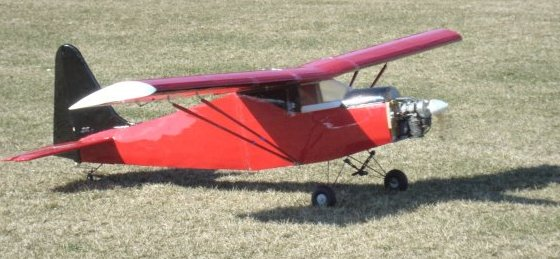
\includegraphics[width=0.5\textwidth]{../images/daedalus.jpg}\\[1cm]
\HRule \\[1cm]
{ \huge \bfseries Rutgers University Autonomous Aircraft Team } \\[0.5cm]
\HRule \\[0.5cm]
{ \large \bfseries Technical Report }
\\[0.5cm]
{ \large \bfseries 2010 AUVSI UAS Competition }
\\[0.5cm]
\HRule \\[1cm]

  {\large Amanda Gaetano, Anthony Garrison, Pat Hickey,}
\\{\large Stephen Indyk, Cogan Noll, John Palmer,}
\\{\large Adrien Perkins, Gregory Quinn, and Michael Varga}
\\[1cm]
\emph{Thank you to our sponsors}
\\ Rutgers University Engineering Governance Council
\\ Rutgers Alumni Association
\\ WINLAB
\\ Invensense, Inc.
\\ ST Micro, Inc.

\vfill
{\large \today}

\end{center}
\end{titlepage}


% We are definitely going to hit the page limit. No more abstract.
%\begin{abstract}
%We will write the abstract after the rest of the paper is finished. 
%If we're really close to the page limit, we may be able to omit it.
%\end{abstract}

\section{Introduction}

The Rutgers Autonomous Aircraft Team was formed in September 2008 with the goal of entering the 2009 AUVSI UAS competition. We didn't make it to the 2009 competition after loosing our aircraft only four weeks before. Our imaging system and autopilot system were also far from ready. 

In terms of NCAA sport eligibility, one could consider 2009 our `red shirt' year. In 2010 we are still rookies.

The team is made of 12 Rutgers undergraduates:\\
\\ \begin{tabular}{l l}
Anthony Garrison, President & John Palmer \\
Amanda Gaetano, Vice President & Adrien Perkins\\
Pat Hickey, Electronics Team Leader & Michael Varga\\
Greg Quinn, Mechanical Team leader & Bradley Lord\\
Stephen Indyk & Taras Wallace\\ 
Cogan Noll & David Wescott\\ \\
\end{tabular}

We are advised by
 Professor Tobias Rossmann,
 and several members of the Tri-County R/C Club \cite{tricountyRC}:
 Larry Kosinar,
 Bill Perkowski,
and  Mike Korb, 
%and Chris (test pilot) 
amongst many who spent time mentoring us.

We have been generously funded by 
Rutgers Engineering Governance Council,
Rutgers Alumni Association, and
WINLAB, a laboratory of the Rutgers University Department of Electrical Engineering.
% What was Chris Brocco's Uncle's Company? Something Automation?
BP Hobbies, 

We would like to acknowledge
Louis Stumpf, for donating the aircraft which became the \emph{Daedalus};
Jeff Perkins, for his prolific networking and promotion of the team;
Gregg Peters of BP Hobbies for getting us out of numerous binds;
Dave Devries and Michael Maia, of Invensense, for their technical guidance;
Professor Chung-chieh Shan, for overseeing Pat's independent study on the IMU design;
Ivan Seskar, for keeping us (and many other undergrads) in the black;
Roger Kondos and Brij Pathak, for contributing to the thermopile attitude sensor.

\begin{figure}[b!]
	\centering
	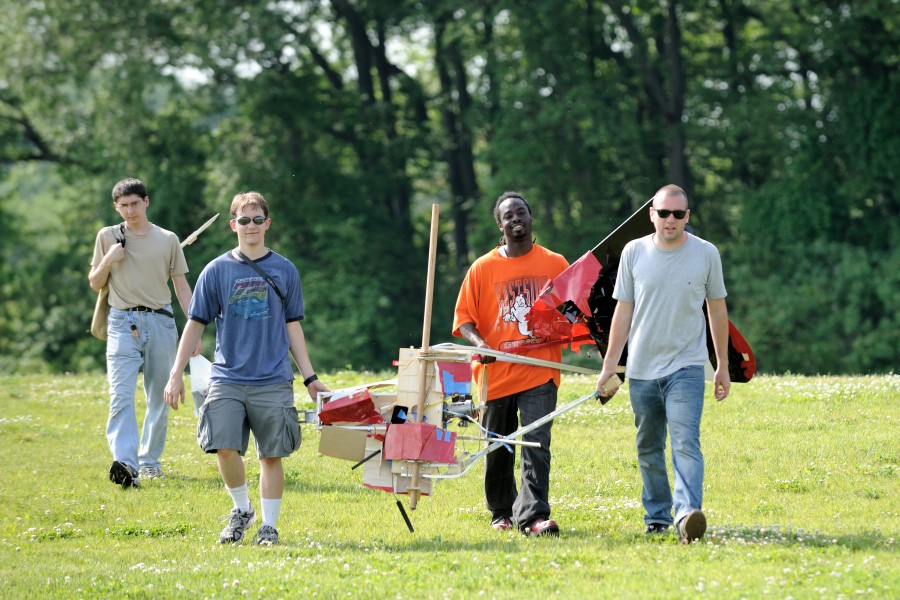
\includegraphics[width=0.6\textwidth]{../images/wreckage.jpg}
	\caption{The recovery of our 2009 entry, the \emph{Icarus}}
	\label{fig:wreckage}
\end{figure}

\newpage
\section{Systems Engineering}
\subsection{Goals}
For this entry, we took a close look at our goals and requirements, and dialed back our approach to ensure we would meet the most basic competition requirements successfully.
We started the design by forming, as a team, some broad goals based on our experience in the 2009 competition.
These formed the basis on which sub-teams and individuals tackled the smaller problems while still keeping an eye on the big picture. 

We also wanted to balance building with buying, keeping in mind our slim finances. While we couldn't build every part of our entry from scratch, we tried to build whatever we could given the 16th June competition deadline.

%\footnote{``If you want to make an apple pie from scratch, you must first create the universe'' - Dr. Carl Sagan \cite{saganquote}}, 


\begin{itemize}
	\item The air vehicle must be stable and slow, with ample payload capacity and 20 minute flight duration. It should be a proven and durable fixed-wing design.
	\item The autopilot must be based on a proven system, so we could focus on improving an existing system rather than reinventing the wheel. It also must be open-source, both because of the high cost commercial systems, and because we want to learn about and experiment with the internals of our autopilot system.
	\item The imaging system must be simple and capable. We assume the operator will be burdened with guiding the camera and identifying targets until time and resources permit us to add sensor information and control loops for guidance, and computer vision for identification. It will be custom built, because we could not find any affordable systems available commercially.
\end{itemize}

We made design decisions of which competition goals we will attempt. 
We will be performing a manual take off, and giving the autopilot system control of the aircraft once the plane is in the air. We will also perform a manual landing. We decided not to pursue the reach goals of autonomous takeoff and landing based on our inexperience and the risk, during development and competition, to our aircraft.
\subsection{System Design Decisions}
\subsubsection{Airframe System Engineering}

Our team was divided by area of expertise into a mechanical team and an electrical team.The mechanical team began the year with the goal of producing two competition worthy airframes. These were to become the \emph{Daedalus} and \emph{Knight Two}.

The teams made design decisions based on the aforementioned competition goals.

One of the most difficult design decisions was to quantify ``ample payload.'' Payload size and weight is the major determining factor in aircraft size.  We originally assumed a 2.5lb electronics (computer + batteries) payload and a 2.5lb pan-tilt camera 8'' in diameter, requiring 6'' of vertical space extruding from the bottom of the aircraft. These considerations introduced two major design parameters: the aircraft must be capable of carrying a minimum 5lb payload, and must be situated to provide clearance for the pan tilt unit.

Additionally, we sought an easily controllable, stable platform to accommodate the autopilot, and an ability to fly at low speeds, in order to more easily capture clear images.

We determined, after consulting with R/C experts, that a high wing trainer is the most stable and proven fixed-wing design. Trainers traditionally have light wing loading for slow speed flight, and are able to carry a comparatively large payload. Additionally, a large plane with lower wing loading is easier to control, and easier to recover if power is lost. Consciously agreeing to err on the side of caution, we sought a large plane capable of accommodating a worst-case scenario payload, and settled on a wingspan on the order of 10'-12'. Though lighter and smaller payload alternatives were found as the year progressed, these merely leave us with more freedom for future modifications.
%That last sentence sounds kind of eh, I'm stuck on a decent wording, so I'm leaving it for now.

The decision to employ a large, high wing trainer, however, forced us to rethink our original pan-tilt design. Last year, in order to accommodate the pan-tilt unit, we designed a pusher plane, enabling us to mount the pan-tilt under the plane's nose, which had sufficient clearance. Since trainers are generally designed with front-mounted engines (I presume?), we were forced to engineer a new solution requiring significantly less clearance. In the long run, we modified the pan-tilt mount to allow us to recess more of the pan-tilt unit into the body of the plane---this had the added benefit of providing more protection to an expensive piece of equipment on takeoff and landing.

\subsubsection{Electronics System Engineering}

The electronics team was in charge of the autopilot system and the imaging system. The biggest system design choice we made was to use a single board Linux-based flight computer as the platform for both systems. We felt that the best way to develop software which interfaces with a wide variety of analog and digital electrical systems, and has complicated information flow requirements.

We had sketched plans for an electronics system built entirely on a Linux-based flight computer as early as July 2009, but planned on using a more standard microcontroller-based autopilot system with an auxillary Linux-based computer for the imaging system until December 2009. After burning out our microcontroller based autopilot for the second time, we were faced with a long lead time for an expensive replacement part. On that impetus, we redesigned our electronics systems to eliminate the microcontroller autopilot and ensure all of our replacment parts would be inexpensive and commercially available from many vendors. The move to a single Linux-based flight computer, while not without obstacles, was a successful design decision, as we'll describe in this paper.

\subsubsection{Autopilot System Engineering}

We felt the Paparazzi system was full featured and proven, but we weren't satisified with the capabilities of the existing Paparazzi hardware. The ``Tiny'' v2.1\cite{paparazzi_tinyv21}, the latest autopilot hardware released by the Paparazzi project, is based on a 64 pin ARM microcontroller. Almost all of its input-output capabilities are dedicated to autopilot functions, making it difficult to expand functionality and share information (for instance, position and orientation estimates) with payload components. As previously stated, the Tiny is expensive, fragile\footnote{In our own admittedly clumsy experience} and often subject to long lead times. 

In order to replace the functionality of the Tiny with a flight computer, we needed to select hardware which could provide the flight control software with information from the attitude sensor, GPS module, and long distance telemetry radio link. We also needed a servo output interface. The most important feature provided by the Tiny was the real-time processing and multiplexing of the safety pilot's radio control signals with the autopilot control signals. The flight computer's servo output hardware must manage this multiplexing functionality in a way that is not tied to the function of the flight computer itself. 

\subsubsection{Safety of Linux Based Flight Computer}

We acknowledge that a Linux based flight computer does not support the requirements for hard real-time, deterministic computing that would be required of any real-world autonomous system. Given the resources available to the team (time, money, and manpower), such a fully assured system is out of reach.

We elected to take many steps in the software engineering to help ensure our flight computer will operate reliably. The most important of these was code review and incremental testing. Both Pat Hickey and Bradley Lord became intimately familiar with the source code and control flow inside the autopilot software, and all patches were reviewed and tested by both engineers. Numerous other safety measures will be described in Section \ref{sec:autopilot_software}.

Because our entry is essentially an experimental system, and will always be operated with a safety pilot present, we engineered the safety pilot override to operate independently from the flight computer. We have ensured that, short of losing power to the radio control receiver and servos, the safety pilot will always be able to take over with the flick of a single switch on his radio control transmitter. We have also ensured that the flight computer's servo controller will be able to detect a loss of computer control and servos to a recoverable default. Along with careful preflight testing, careful observation, and definitive analysis of any errors encountered during flight, these measures meet the spirit and letter of competition rules.

\subsubsection{Imaging System Engineering}

When designing the imaging system our major goals were to have 1) a camera with XXX range of motion.  2) real-time video feed from the plane.  3) ability to control the camera in real-time and take pictures.  4) ability to download pictures while in flight.  For the camera we chose the Sony Bloggie \cite{bloggie} because it was small, light, cheap, and took high resolution images and video.  In addition it came with a built in rotating lens, which simplified the construcion of the pan-tilt unit, and it can also be controlled remotely over usb, so it interfaced with our flight linux computer.  To communicate with the plane we developed custom ground station software to meet our needs and installed two sets of radios, one for the video feed, and another for communicating with the plane and downloading images.  These radios are independent from the set of radios used for the autopilot because we didn't want to have dependencies between the two systems.

\section{Flight Vehicle}

At the time of this writing, we have completed and flown a single flight vehicle, which we have named the \emph{Daedalus}.
We have also nearly completed a very similar backup airframe which serve as a backup in case the \emph{Daedalus} has a disaster. The \emph{Knight Two} will be fitted with nearly identical R/C flight electronics, and accept the same autopilot and imaging system payload as the \emph{Daedalus}.

\subsection{Airframe}

We elected to pursue a kit-type airplane rather than our own design. 
Our own custom design, the \emph{Icarus}, suffered a catastrophic structural failure last year. From this, we learned that custom structures require much more testing and revision than a proven kit. We also reconsidered our payload requirements and decided we could easily modify a kit plane to accept our autopilot and imaging system.



\subsubsection{Daedalus}
\begin{wrapfigure}{l}{0.4\textwidth}
	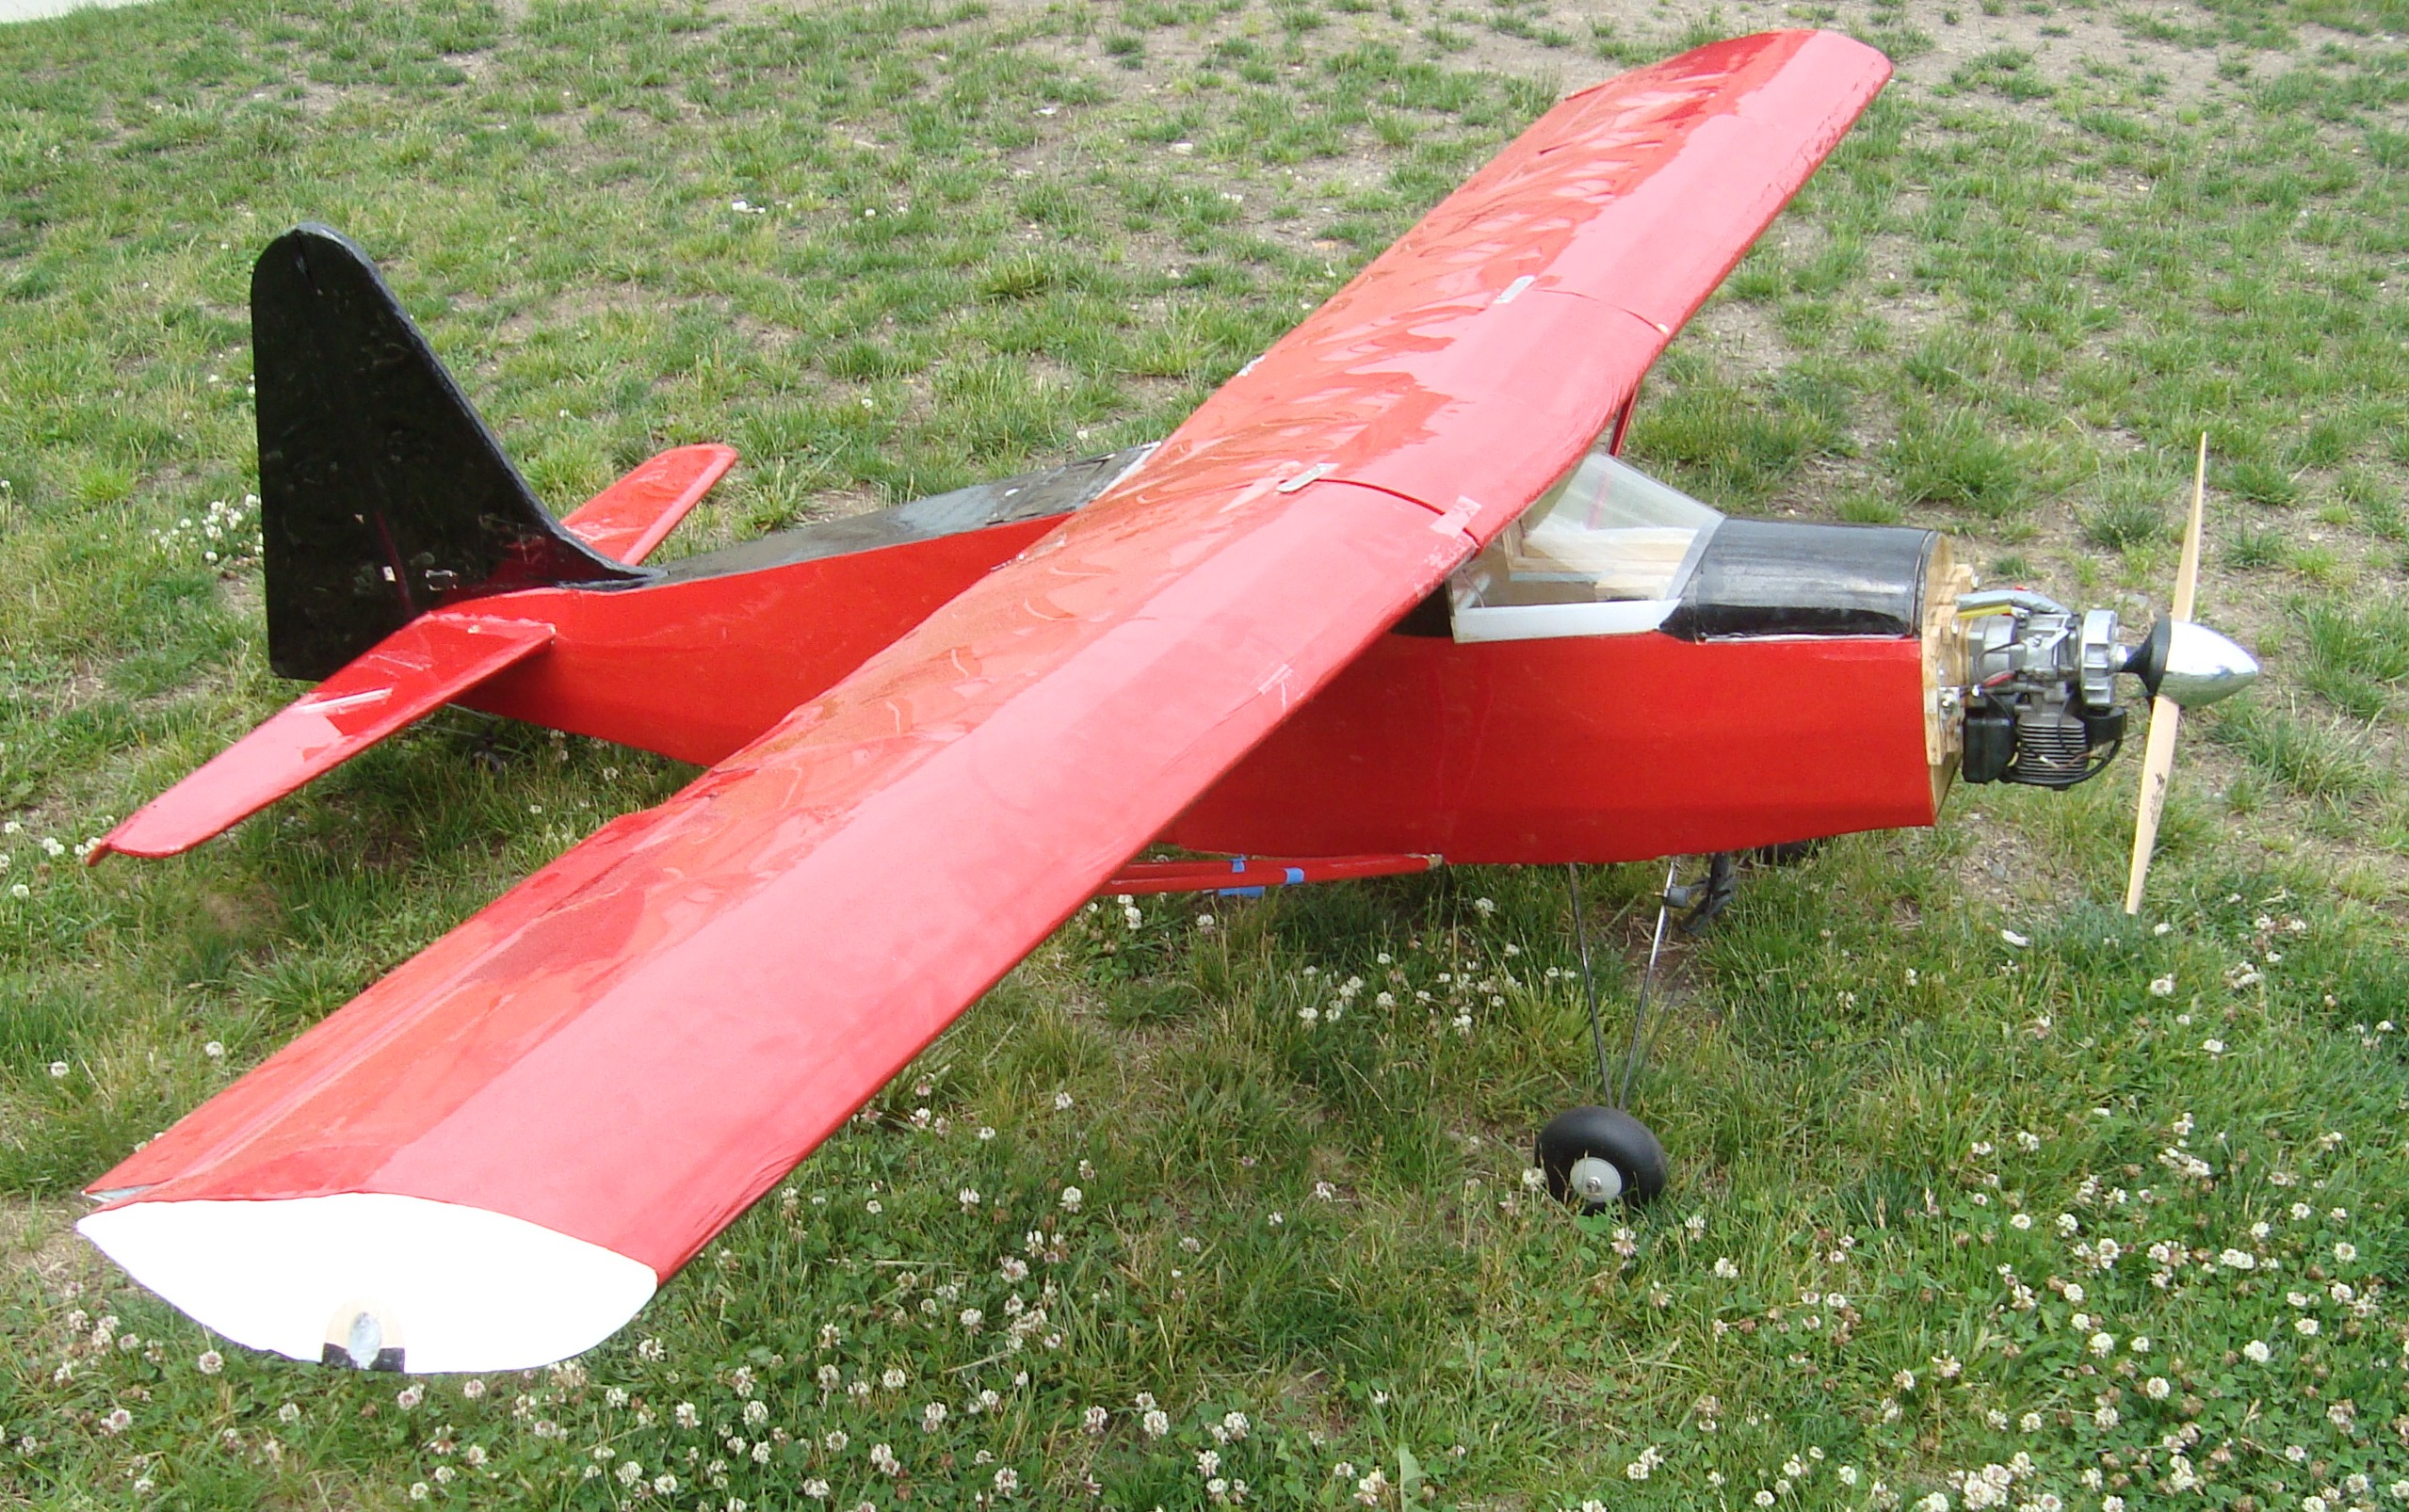
\includegraphics[width=0.37\textwidth]{../images/daedalus_isometric.jpg}
	\caption{The \emph{Daedalus}}
	\label{fig:daedalus}
\end{wrapfigure}
A member of our local R/C club, Tri-County RC \cite{tricountyRC}, donated a ten-foot wingspan high wing trainer to our club. The plane, first built out of foam and balsa from long-lost plans in 1986, was accepted graciously, but required quite a bit of work before it was once again flight-worthy. We removed the covering to find water damage and rot which resulted from years of storage. We stripped and rebuilt nearly the entire airframe, adding carbon-fiber reinforcements to the wing in anticipation of increased wing loading due to our payload. Once rebuilt and covered, we tested the \emph{Daedalus} weighed 19.5 lbs with engine. A full 24oz fuel tank, plus 3.5 lbs electronics payload, would bring the maximum takeoff weight to 25.5lbs.

We wanted to certify the wings and wing root would withstand large dynamic forces in flight. 
We designed a test similar to mimic the 
Federal Airworthiness Standards' structural requirements\footnote{Special Federal Aviation Regulation No. 23, Subpart C--Structure. Assuming full load on wing as described in 23.335 paragraph 4.i., where an aircraft must pull out of a \degrees{7.5} dive at cruise velocity and cruise power ``with a load factor of 1.5 (0.5$g$. acceleration increment)'' \cite{far23}}. Our first test was designed to certify that the wing, supported at the wing root and fuselage, could take a bottom loading present in a 1.5$g$ acceleration, with a safety factor of 1.5\footnote{As stated in 23.303 \cite{far23}.}.

 \begin{wrapfigure}{r}{0.4\textwidth}
	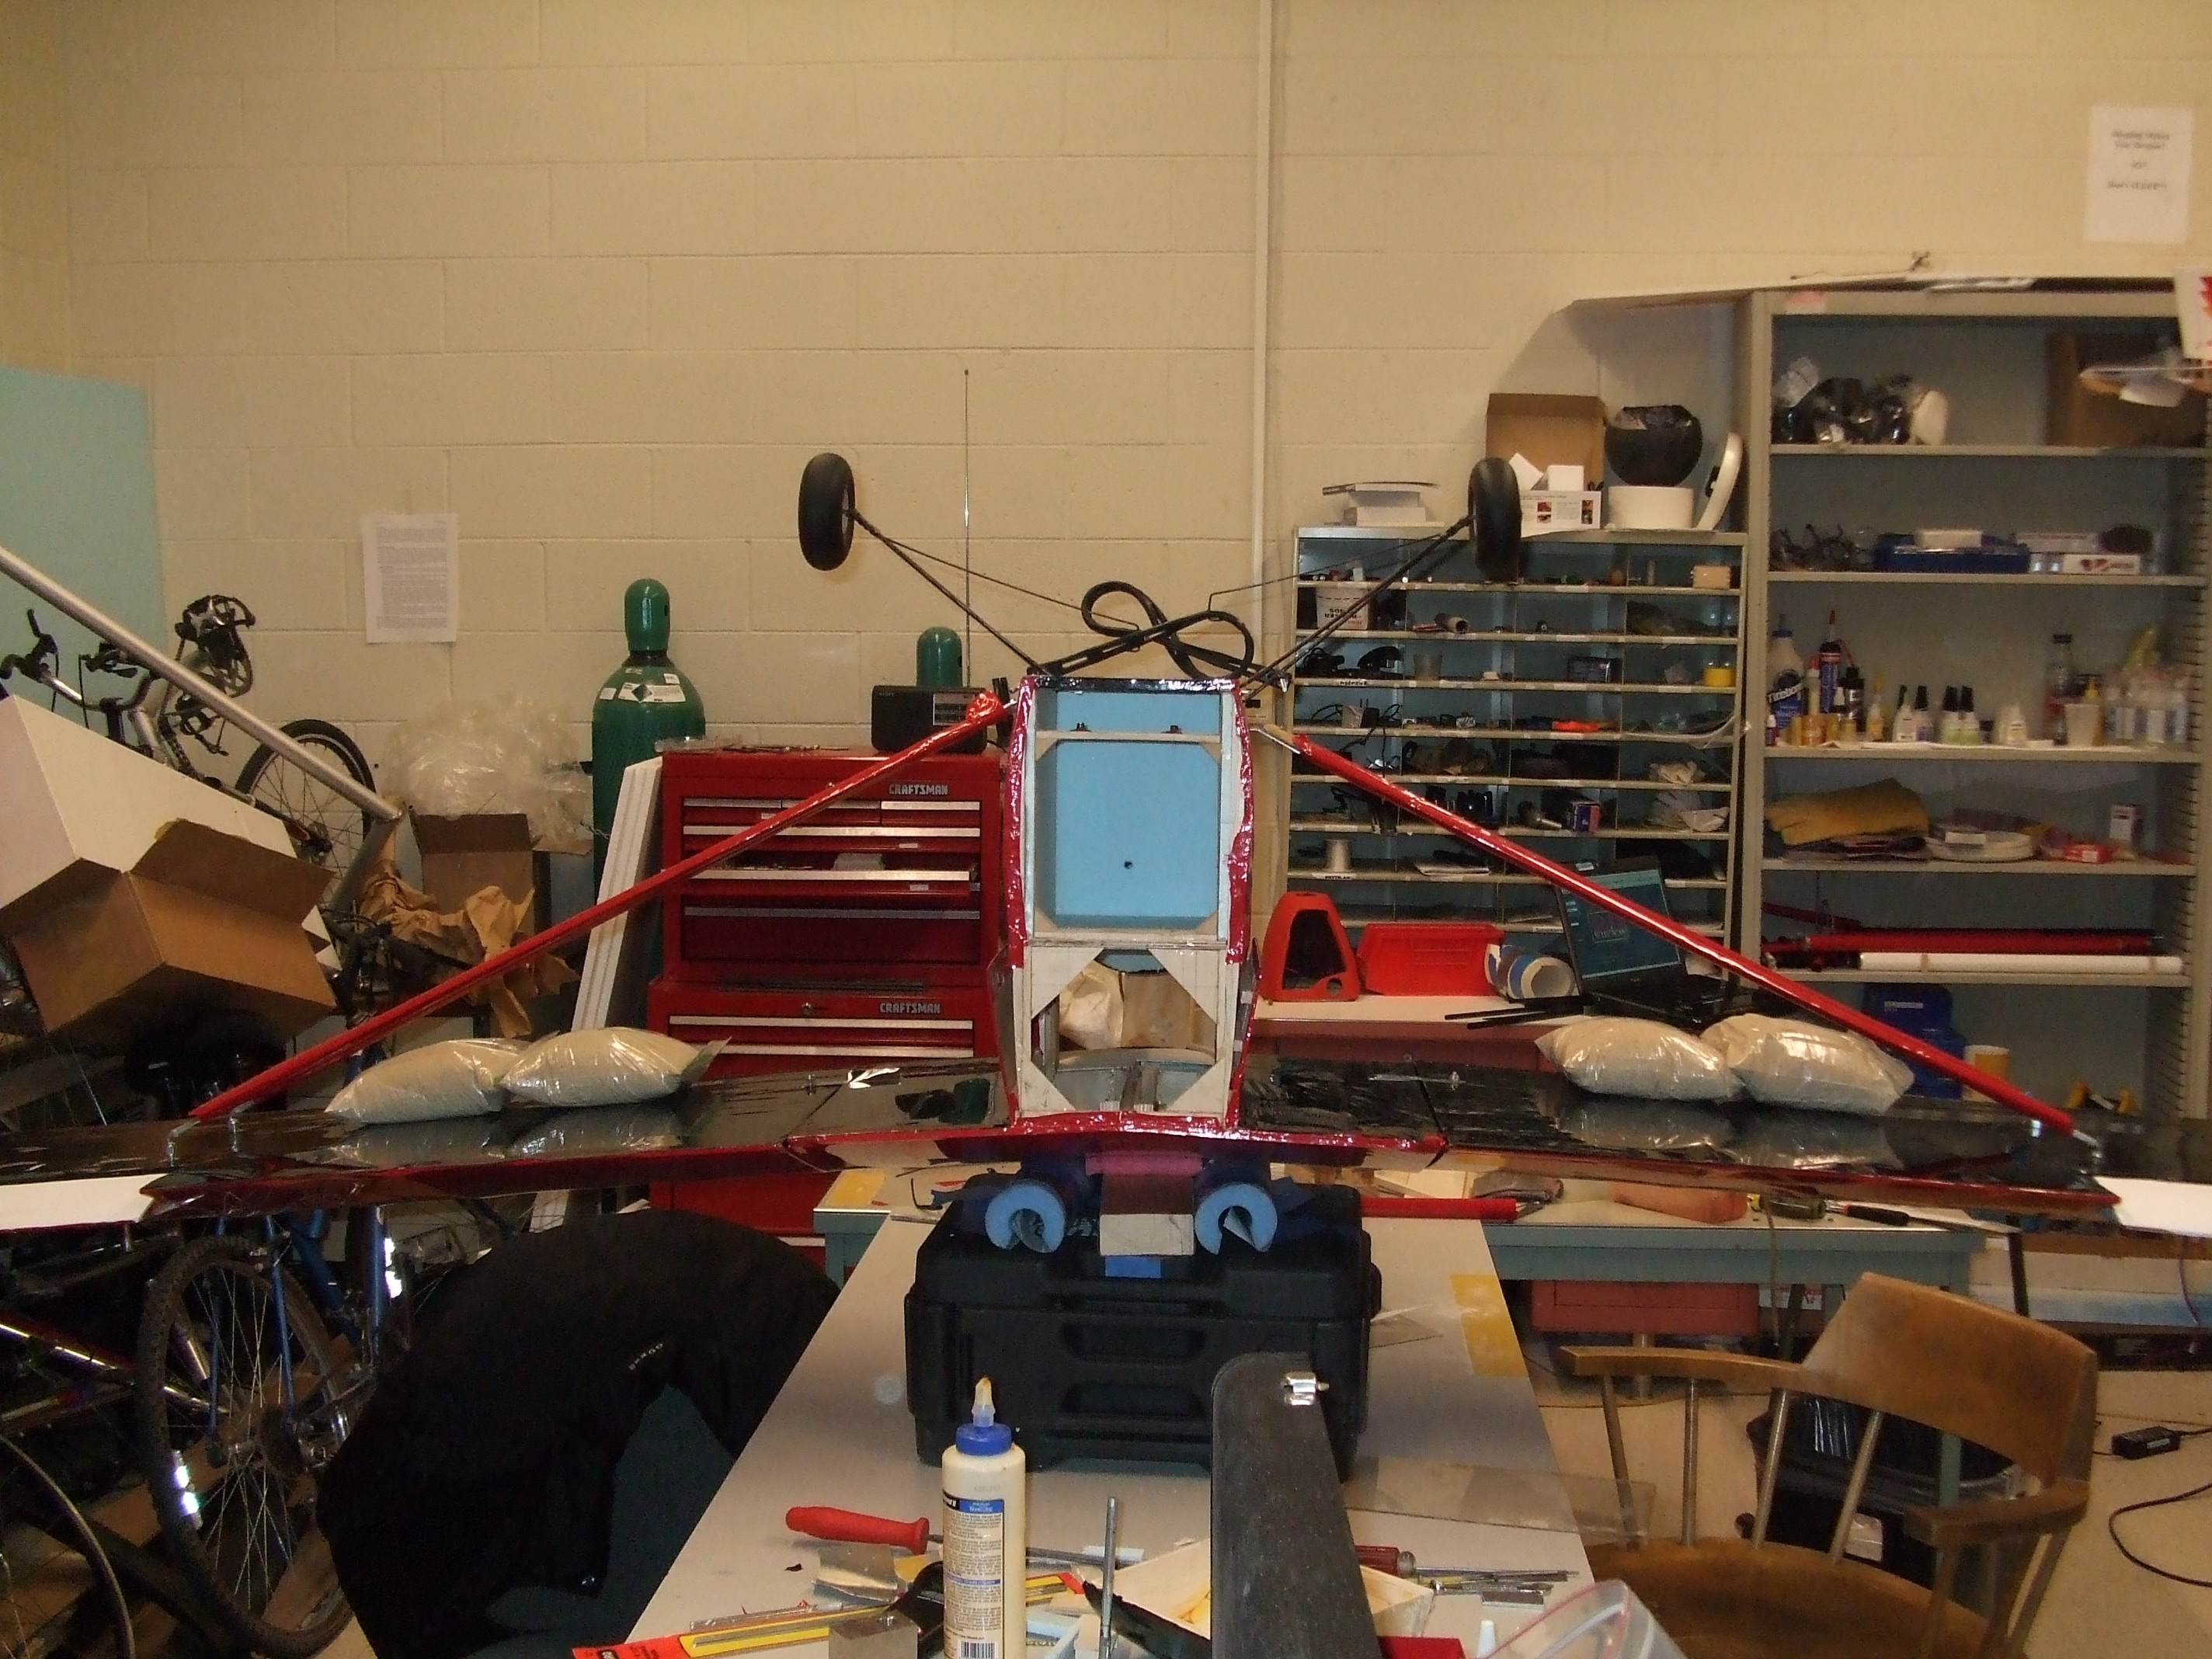
\includegraphics[width=0.37\textwidth]{../images/daedalus_sandbagtest.jpg}
	\caption{Load testing the underside of the \emph{Daedalus}'s wings. Shown with 16lbs of load.}
	\label{fig:sandbagtest}
\end{wrapfigure}
The plane was carefully supported under the center section, nose, and tail while pre-weighed bags of sand were slowly placed symmetrically and simultaneously on the underside of each wing, starting from the innermost rib.  The \emph{Daedalus} wings supported 64 lbs (250\% of the maximum take-off weight) under static loading.  We also rocked the plane ten degrees from side to side while fully loaded to simulate differential loads during flight. Our post-test structure inspection found no warped members or cracked joints.

A second test was designed to certify the wing could take a top loading present from a 1.5$g$ acceleration with a safety factor of 1.5, and to certify that load could be transmitted to the ground through the fuselage and landing gear. With the aircraft fully assembled and sitting upright on the landing gear, we loaded the top of the wing along the quarter chord with 64 lbs of sandbags. As in our first test, we also rocked the plane \degrees{10} side to side to simulate uneven loading. Our post-test structure inspection once again found no warped members or cracked joints.

Satisfied, made engine and surface tests (see \ref{sec:appendix_preflight}) before taxiing the plane around a parking lot.  We brought the plane back inside, examined it for signs of stress and, finding everything in good condition, deemed the \emph{Daedalus} flight-worthy.

\begin{wrapfigure}{l}{0.4\textwidth}
	\centering
	\subfloat[The unfinished \emph{Knight Two}]{\label{fig:knighttwo_construction} 
			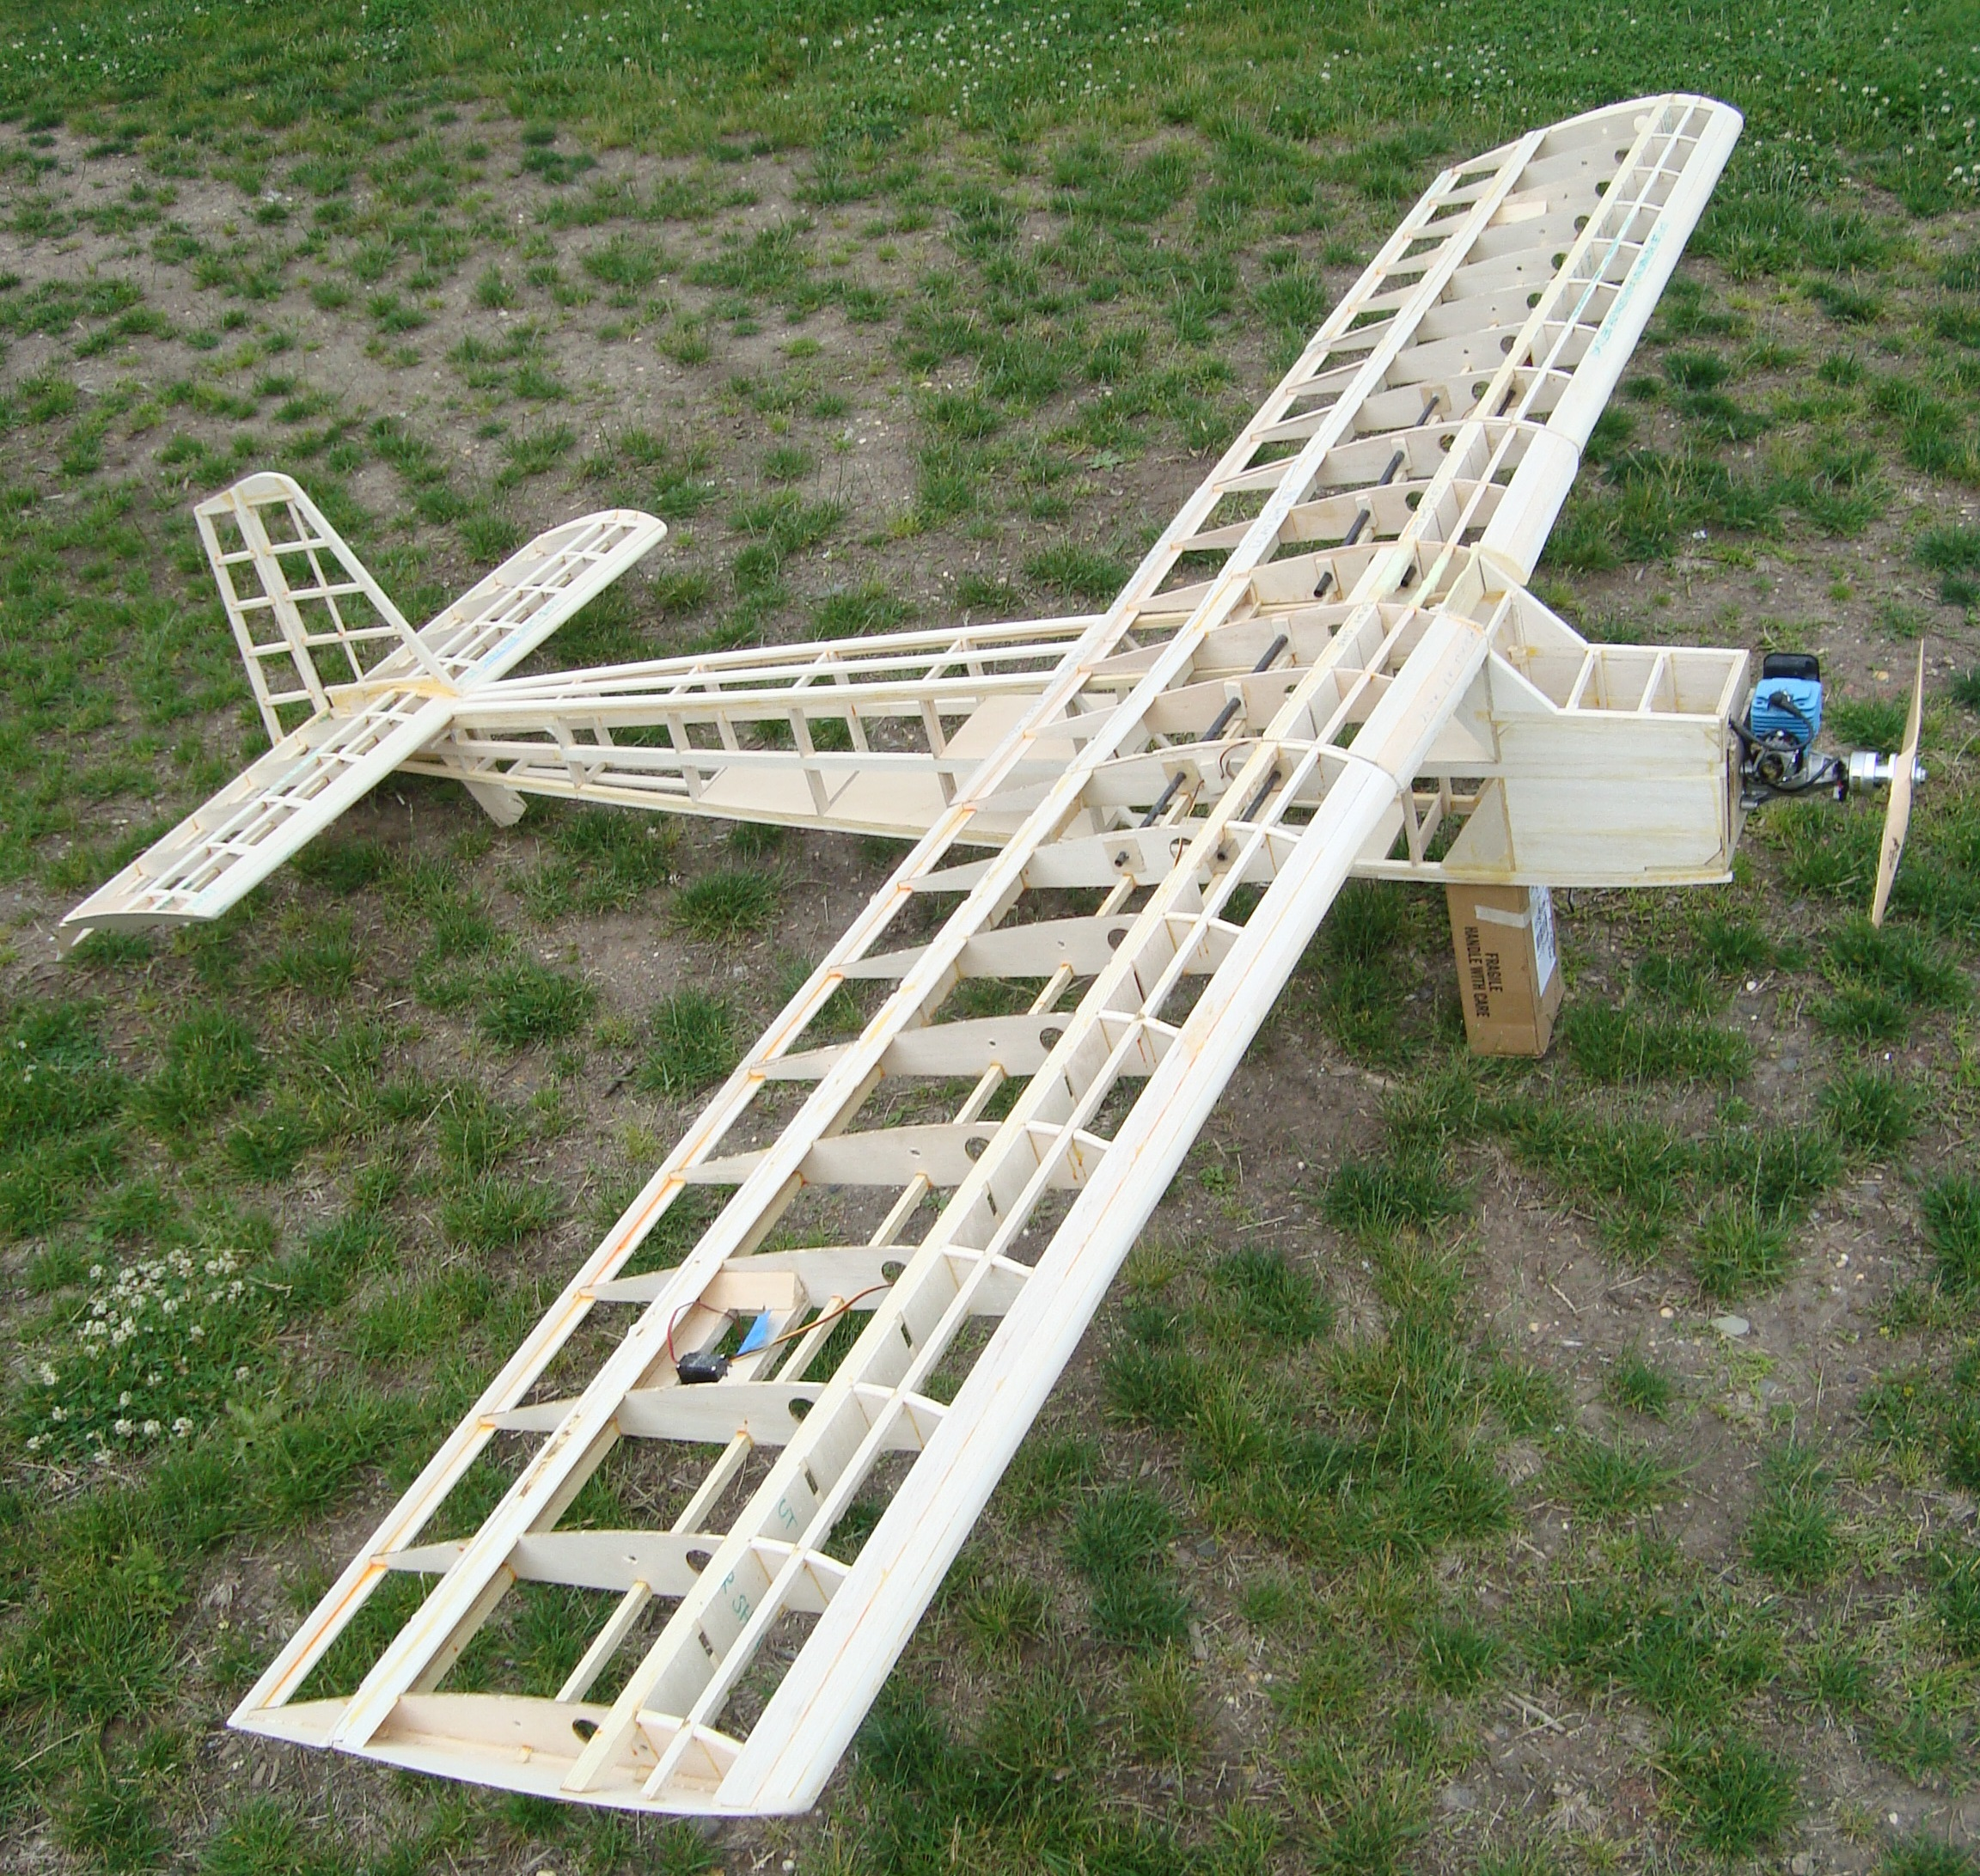
\includegraphics[width=0.37\textwidth]{../images/knighttwo_uncovered_outdoors.jpg}}
\\
	\subfloat[A completed 12 Foot Telemaster. Photo Credit: Hobby Lobby] {\label{fig:knighttwo_12ft_telemaster} 
			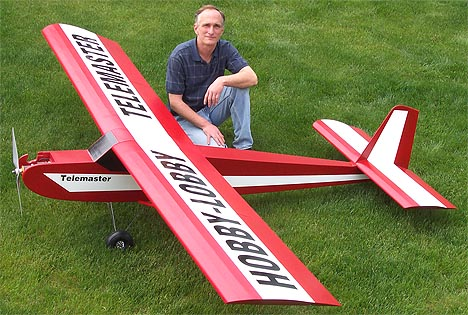
\includegraphics[width=0.37\textwidth]{../images/telemaster_12ft_hobbylobby.jpg}}
  	\label{fig:knighttwo}
  	\caption[Knight Two]{Knight Two}

\end{wrapfigure}
Someone please detail the outer dimensions. The inner dimensions, space used for flight electronics, space used for payload underneath. Landing gear height. Number of servos and their locations

\subsubsection{Knight Two}

In order to mitigate a disaster such as we had last year, we decided to build another airframe which could replace the \emph{Daedalus} at short notice. We selected an Aero-Design 12 Foot Telemaster \cite{aerodesign} because it was available as a balsa kit and similar in size to the \emph{Daedalus}.

We named it the \emph{Knight Two} after the Rutgers University mascot, the Scarlet Knight. We may rename it if someone can think of a better name. Pat needed to think up a decent name real fast in order to make this rough draft.

Since our testing plan for the \emph{Daedalus} was successful, we will follow the same plan when, in the coming weeks, we finish building \emph{Knight Two}.


Someone please detail the outer dimensions. The inner dimensions, space used for flight electronics, space used for payload underneath. Landing gear height. Number of servos and their locations

Figure may go here: Line drawing of Knight Two. JOHN

\subsection{Power}

\subsubsection{Engine}

Each airframe has a 45cc gasoline engine and 24 ounce gasoline tank. Based on our flight tests, with climbs to 400 feet AGL and a high throttle cruise, we use a little less than 1oz gasoline per minute. While actual fuel consumption may be less, we set a flight time cap at 20 minutes in order to always have a safety reserve of at least 4oz. We have tested to ensure that, within \degrees{\pm10} of level flight, the fuel tank will feed the engine until less than $1/2$oz fuel remains.

\subsubsection{Batteries}

Each airframe has nearly identical flight electronics. To power a Futaba 2.4GHz receiver and 6 servos for a 20 minute flight, we selected a 2 cell (7.2v) 3.2 amp hour Lithium Ion battery with a 5v, 10A capacity switching regulator made by Castle Creations. We use a low voltage monitor in-line with the battery, which beeps when cell voltage falls below 7.2v. The autopilot electronics are powered off a completely separate battery for safety.

\section{Autopilot}
Our entry uses an autopilot system based off the open source 
Paparazzi project\cite{paparazziweb}. 
We ported the airborne code to Linux in order to use a single computer for all of our flight hardware and software.

\subsection{Requirements}

We needed to interface with the following hardware components:
\begin{itemize}
	\setlength{\itemsep}{0cm}
	\setlength{\parskip}{0cm}
	\item GPS
	\item servos
	\item camera
	\item etc.
\end{itemize}

Interfacing with such a large array of devices meant we had to use a ...

\subsection{Hardware}
Single board computer: beagleboard.

Description of each input, output interface.

Figure goes here: Hardware connection diagram. PAT
\subsection{Software}
\label{sec:autopilot_software}
PAT

Figure goes here: interprocess communication. PAT
\subsection{Ground Station}
Because we based our autopilot software on the Paparazzi project, we were able to make use of their excellent ground control software (GCS) with essentially no modifications.

Detail the capabilities of the Paparazzi GCS.

Figure goes here: Paparazzi ground station screenshot, or whatever. 
\subsection{Tuning and Testing}
PAT

\section{Imaging System}

To obtain images of targets in flight we have created an Imaging System capable of meeting all the requirements of the competition.  The system consists of a pan-tilt camera on the plane, communication software on the plane, and our ``Image Station'' application running on a dedicated laptop.  The Image Station communicates with the plane in real time via two different sets of wireless radios.  Using the Image Station, the operator can view a live video stream from the plane, control the pan-tilt camera remotely, and download and manipulate images.

\subsection{Camera}
\begin{figure}
	\centering
	\subfloat[Front View]{\label{fig:camera_frontview} 
			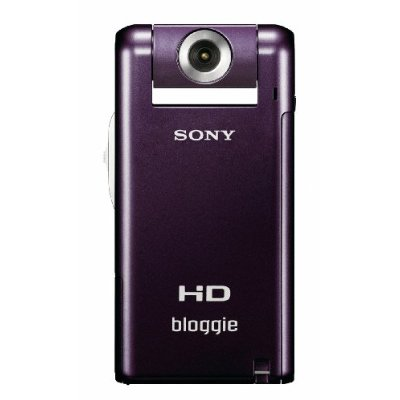
\includegraphics[width=0.3\textwidth]{../images/camera_frontview.jpg}}
	\subfloat[Isometric View]{\label{fig:camera_isometric} 
			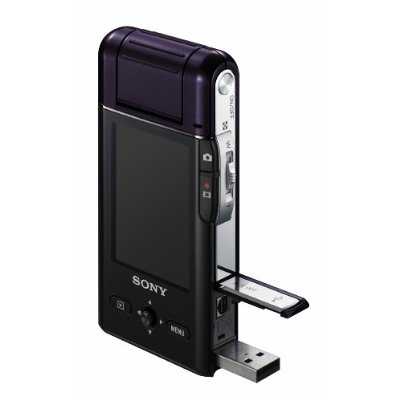
\includegraphics[width=0.3\textwidth]{../images/camera_isometric.jpg}}
	\caption{Sony MHS-PM5. Image Credit: Sony}
	\label{fig:camera}
\end{figure}

We selected the Sony MHS-PM5 camera as the basis of our imaging system. Marketed as a pocket 1080i video camera capable of 5 megapixel (MP) still images, we primarily selected the camera because it features a swiveling lens at one end of the body and it features Sony's LANC (Local Application Control Bus System, ref{lanc}). Because the swiveling lens is at one end of the body, we can mount the camera primarily inside the fuselage of the aircraft, which will protect it from damage on takeoff and landing. Internal mounting also helps reduce drag. The swiveling lens is an important feature because it allows us to achieve two rotational degrees of freedom while only rotating the body about one axis. This simplifies the pan tilt unit design.

The LANC protocol is based on a 9600 baud UART serial connection, and is available on the PM5's 10-pin ``Multi-AV'' connector. Camera control commands, which include commands to zoom in, zoom out, and take a still picture, is publicly available \ref{boehmenl_lanc}. Also on the ``Multi-AV'' connector are the signals for NTSC video and audio output. We use both the NTSC output and LANC signals on this connector using a commercially available adapter cable \ref{lanc_multiav_cable}.

% first citation should go to http://www.boehmel.de/lanc.htm

The PM5's NTSC video signal outputs a 480 line video of the current ``viewfinder'', the live video that is also displayed on the rear LCD screen. 
Still pictures are taken based on targets spotted in this video feed and are stored on the camera's memory card.

Each still picture is 5 megapixels, with an actual resolution of 2592 x 1944.  To determine how the images will appear from different altitudes, we have a table that maps the size of features in the world to pixels in our images at different altitudes.  We also see how this mapping will be affected when the camera is pointed straight down compared to when it is tilted at a 45 degree angle.  We can see that at 100 ft. each pixel will represent a little over $1/3$ of an inch when looking straight down, which should be a sufficient level of detail to accurately identify any target.  However, at 500 ft. each pixel is 2 inches wide when looking straight down, which will lead to blurry images.  We are confident that this level of detail will be enough to identify the shapes and colors of all targets at any required altitude, but we may have some difficulty identifying alpha-numerics on very small targets at high altitudes.  As a first year team, we feel that this is an acceptable level of detail.

\begin{tabular}{ccc}
{\bf altitude (ft)} & {\bf pixel width at $0,^{\circ}$ (in)} & {\bf pixel width at $45,^{\circ}$ (in)} \\
       100 &       0.38 &       0.54 \\
       200 &       0.76 &       1.08 \\
       300 &       1.14 &       1.62 \\
       400 &       1.52 &       2.16 \\
       500 &       1.90 &       2.69 \\
\end{tabular}

% please give details of still pictures, including the field of view per pixel. include a quick table of resolving power (projection of pixel field of view, center of frame, onto ground) at altitudes [100,200,300,400 agl] for straight down and 45 degree angle. Please also give the resolving power of the video viewfinder

\subsection{Pan Tilt Unit}

\begin{figure}
	\centering
	\subfloat[Isometric View]{\label{fig:pantilt_isometric} 
			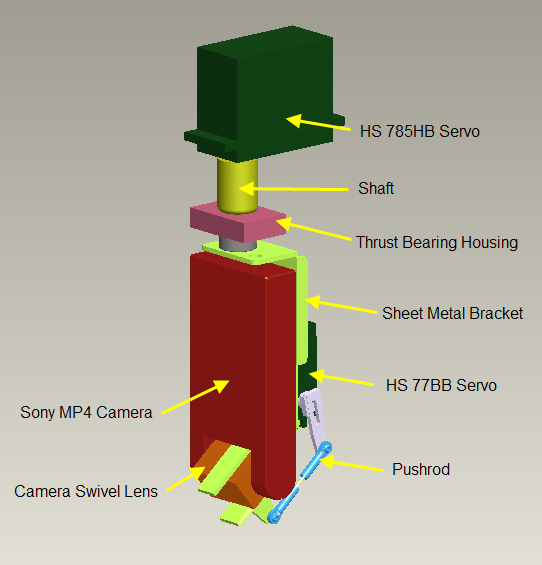
\includegraphics[width=0.75\textwidth]{../images/pantilt_isometric.png}}
\\
	\subfloat[Side View.]{\label{fig:pantilt_side} 
			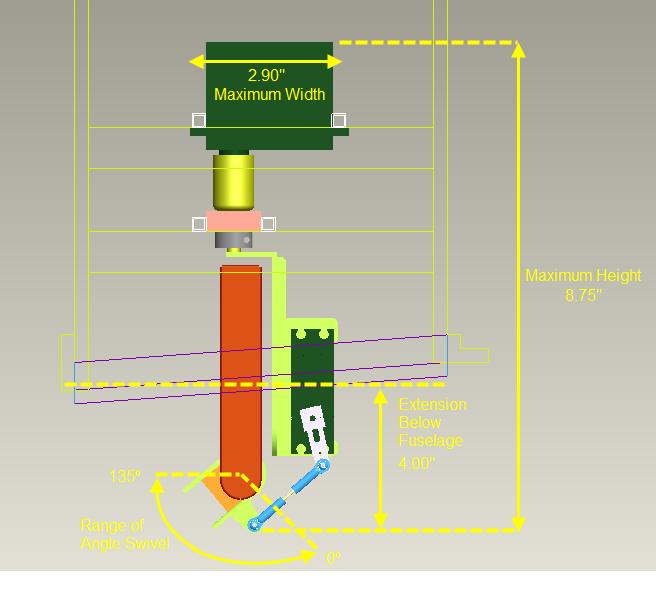
\includegraphics[width=0.75\textwidth]{../images/pantilt_side.png}}
	\caption{Pan Tilt Unit}
	\label{fig:pantilt}
\end{figure}
\begin{figure}
	\subfloat[Linkage Detail View]{\label{fig:pantilt_linkdetail} 
			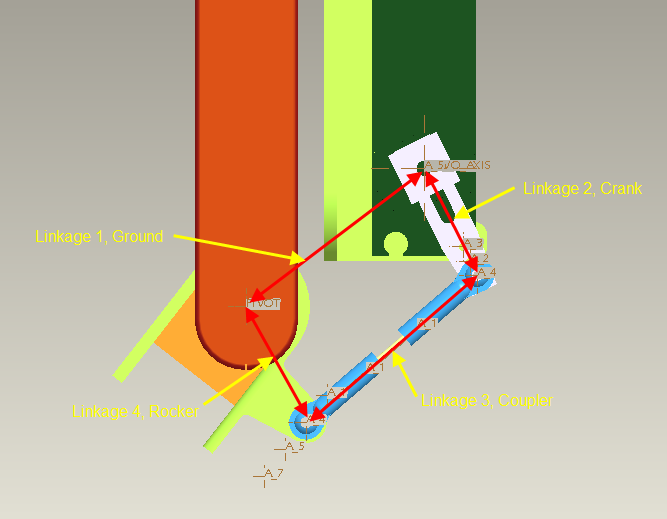
\includegraphics[width=0.6\textwidth]{../images/pantilt_linkdetail.png}}
	\subfloat[Linkage Velocity Plots]{\label{fig:pantilt_linkplots} 
			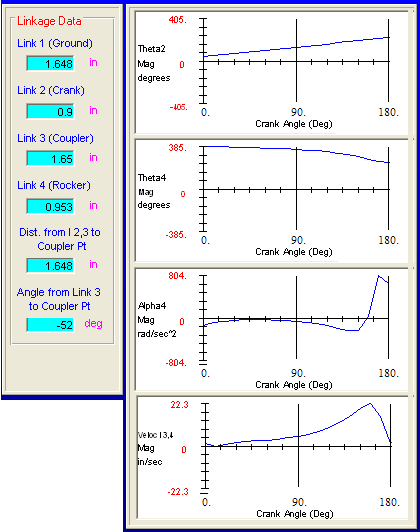
\includegraphics[width=0.4\textwidth]{../images/pantilt_linkplot.png}}
	\caption{Tilt Linkage Detail}
	\label{fig:pantilt_link}
\end{figure}

In order to meet the target imaging requirments, we needed to add both pan and tilt actuators to the camera. The XX by YY degree lens field of view is insufficient to see off flight path targets, and would limit our capability in the target search area phase. 
We designed a pan tilt unit which make it possible to image the entire hemisphere below the fuselage of the aircraft.

We took advantage of the MHS-PM5's swiveling lens assembly 
(see Figure \ref{fig:camera_frontview}, and added a servo actuator which could rotate the lens \degrees{135} back from straight forward, as shown in Figure \ref{fig:pantilt_linkdetail}. The tilt servo is a Hitech HS 77BB \ref{hitechs77bb}, and is capable of \degrees{180} rotation. Figures \ref{fig:pantilt} and \ref{fig:pantilt_linkdetail} show the camera lens tilted at \degrees{45} below the horizon.
The camera and tilt servo assembley is attached to the aircraft on a rotating mount. A thrust bearing takes lateral loads off the pan servo shaft, and stabilizes the assembly. The pan servo is a Hitech HS 785HB \ref{hitechhs785}, and is capable of \degrees{1260} rotation (3.5 revolutions). Both servos are powered and controlled by the Pan-tilt control board.

The total height of the imaging system is 8.75", only 4'' of which is exposed below the fuselage of the aircraft. The rotating assembly is, on its widest dimension 2.13", and would fit inside a 2.5" cylinder. Wires exiting the side of the camera, inside the fuselage, may make the assembly a bit wider. Because the maximum rotation is only \degrees{1260}, the camera and tilt servo wires only have to be capable of wrapping \degrees{\pm 630} around the shaft below the thrust bearing. A wire guide will be added to keep the wires from tangling once construction of the pan-tilt is complete and installed in the aircraft. 

The pan servo is calibrated before installation by mapping servo PWM inputs to a measured angular output at \degrees{30} intervals. Linear interpolation is used to determine PWM outputs which achieve intermediate angles. The tilt servo is calibrated at \degrees{10} intervals, due to its much smaller rotation range. As shown in Figure \ref{fig:pantilt_linkplots}, the angular acceleration of the camera angle linkage (Alpha4) is almost constant compared to the servo arm linkage throughout the range $[0^{\circ}, 135^{\circ}]$. The linkage has been designed to keep the majority of nonlinear rotation outside the camera's range of rotation. Therefore, we can consider the calibrated servo output to be directly related to the camera angle.
The endpoints of the tilt rotation rang are calibrated and enforced in software, because pushing the camera outside this range may damage it.

\subsection{Obtaining Images}

The entire imaging system is controlled by the ``Image Station Operator''.  They view a live video stream coming from the camera on the plane, which is transmitted over a high bandwidth radio.  The operator can also control the camera by sending commands to the plane over the XBee radio link.  In order to assist the operator in finding targets, a target locating algorithm will be run on the video feed to highlight possible targets.  At the time of writing work is in progress on this feature, and it is being implemented using the OpenCV library \cite{opencv} with contour detection and polygonal mapping functions.

\begin{figure} [H]
  \centering
  	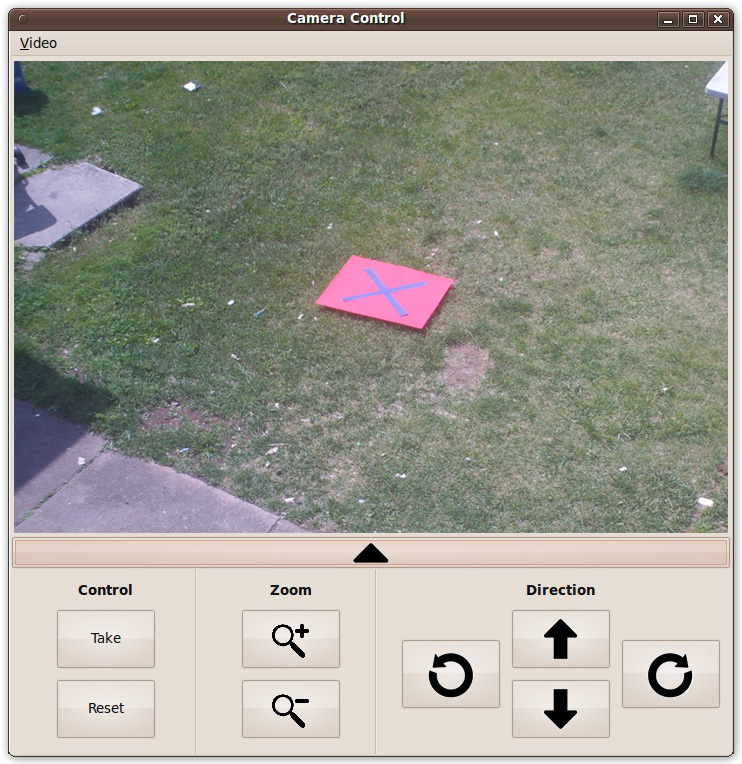
\includegraphics[width=0.9\textwidth]{../images/ImageStationControls.jpg}
  	\caption[Image Station Control Panel]{The Control Panel for the Image Station.  Above is a live video feed from the plane.  Below are controls to adjust the pan/tilt of the unit, zoom in/out, take a picture, and reset the camera to a neutral position.}
  	\label{fig:imagestationcontrols}
\end{figure}

When a picture is taken on the plane it is immediately saved on the camera's memory card.  In order to view that picture on the ground it must first be transferred to the plane's main computer (beagle board).  This is done via the PM5's USB connector.  When attached to a computer, the PM5 powers the camera off and appears as a USB Mass Storage Device. In order to use the PM5 as both a camera and Mass Storage Device in flight, we have spliced a transistor into the power line on the USB cable. This controls whether the camera detects it is connected via USB by blocking or allowing current in that line.

\subsection{Downloading Images in Real Time}

Once images are on the plane's computer they are ready to be downloaded over a 2.4GHz XBee radio link.  Each picture taken by the camera is about 500KB in size, while our theoretical maximum throughput is only 115200 baud (and only about half of that in practice).  Each full image takes about a minute to download, so we created a method to speed up the process.  The entire image is first downloaded as an 800x600 resolution `thumbnail.'  Once the thumbnail is available for viewing, the operator can select an area of interest and download a high-res crop of just that area.  Downloading both the crop and the thumbnail generally takes under 30 seconds, less than half the time of downloading the full image, allowing us to quickly obtain high resolution images of the targets of interest.

\begin{tabular}{rrr}
 & {\bf Size (KB)} & {\bf Download Time (s)} \\
 {\bf Original Image} &        500 &       69.4 \\
 {\bf Thumbnail} &        125 &       17.4 \\
 {\bf Crop} &         25 &        3.5 \\
\end{tabular}

Below a diagram is included that shows the entire flow of events from start to finish in our Imaging System for capturing an image and then downloading it.

\begin{figure} [H]
  \centering
  	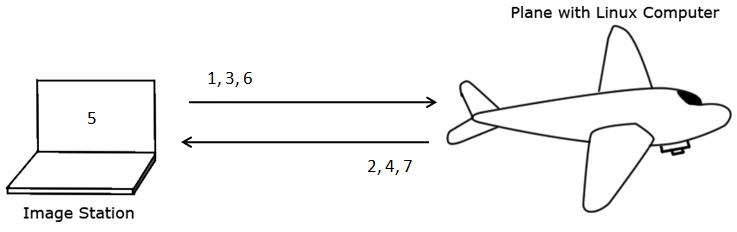
\includegraphics[width=0.9\textwidth]{../images/CaptureProcess.jpg}
  	\caption[Image Capture Process]{Flow of events for capturing an image}
  	\label{fig:imagecaptureprocess}
\end{figure}

\begin{enumerate}
\item Command to take a picture is sent to Plane from Image Station
\item Plane sends command to camera, picture is taken and acknowledgement is sent to Image Station
\item Operator issues command to make images available for download
\item Plane acknowledges request and begins transfer of images from internal camera memory to the BeagleBoard.  Sends notification when transfer is complete.
\item Newly available image(s) are automatically put on a queue to be downloaded.
\item A request to download a 250 byte chunk of the image at the top of the queue is sent to the plane.
\item The plane sends down the requested chunk of image.
\item Steps 6-7 are repeated throughout the duration of the flight.  These image downloading commands are low priority and will only be sent if there are no other commands to be executed, This allows for high priority commands like taking a picture or moving the camera to be executed at any time.
\end{enumerate}

\subsection{Identifying target characteristics}

When an image has been fully downloaded to the ground targets can be identified and tagged with metadata.  Information about the plane's orientation, gps coordinates, altitude, yaw/pitch/roll, and pan/tilt of the camera are sent down with the image.  Using this information the GPS location of the target can be determined using the intrinsic properties of the camera and some basic trigonometry. Target shape, color, alphanumeric, alphanumeric color, and orientation are all entered manually by the operator.

\begin{figure} [h]
  \centering
  	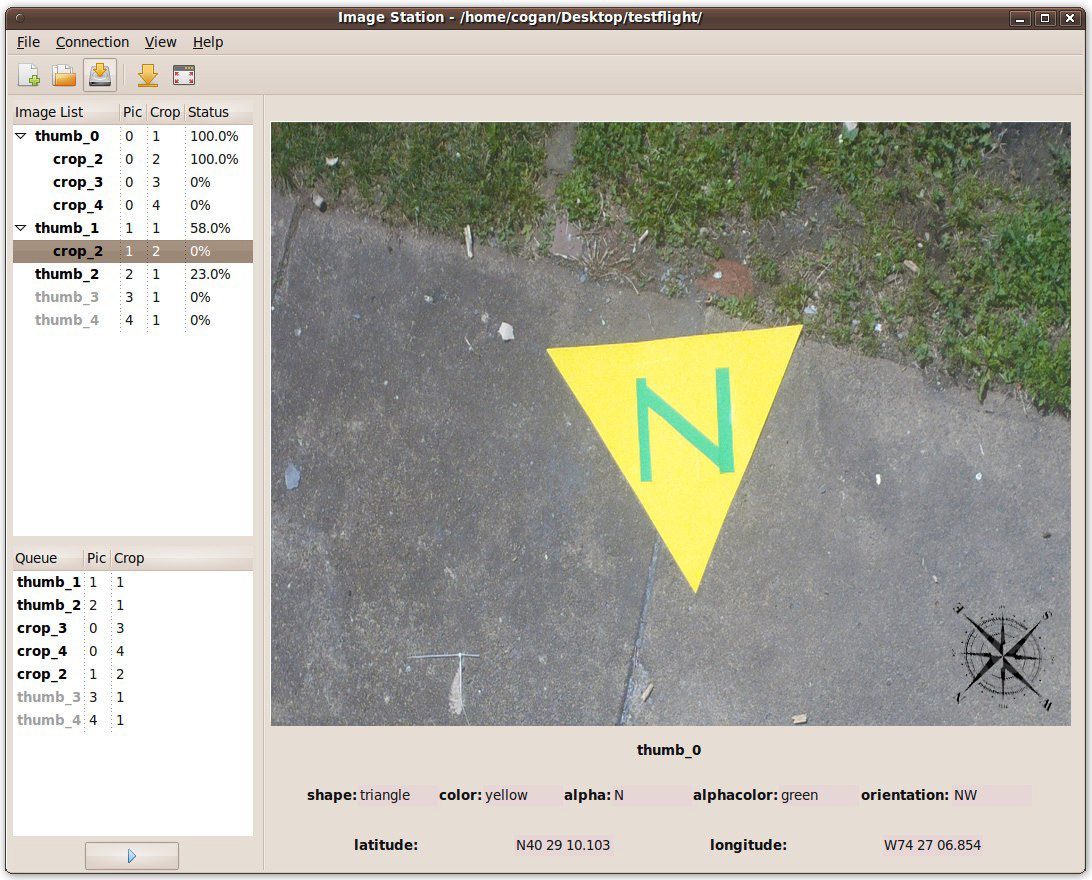
\includegraphics[width=0.9\textwidth]{../images/ImageStationMain.jpg}
  	\caption[Image Station Interface]{The main interface for the Image Station.  All the images that have been taken are displayed on the top left.  The queue of images to download is on the bottom left.  On the right is the currently displayed image, with target information underneath.}
  	\label{fig:imagestationinterface}
\end{figure}

\section{Operation Safety}

We consider the safety of our team, our aircraft, and our spectators to be of utmost importance.  As such, we've implemented numerous safety features and developed a strict procedure for starting, taxiing, and flying the plane.  This procedure enables us to ensure that all personnel are safely in place, and that no integral checks are missed.

\subsection{Safety Features}
Our system is designed to gracefully handle any failure while continuing to ensure the safety of those nearby. 
\begin{itemize}
	\setlength{\itemsep}{0cm}
	\setlength{\parskip}{0cm}
	\item Channel 5 (?) allows quick switch to safety pilot in case of autopilot malfunction.
	\item If the plane loses contact with the ground station for more than XX seconds, the autopilot will default to a ``return home mode'' that will direct the plane towards the ground station in hopes of reestablishing a connection.  If the connection remains dead for XX minutes, the autopilot will direct the plane to [DO SOMETHING?]
	\item Channel 6 (?) functions as a remote kill switch, ensuring the ability to cut power to the engine if an emergent situation precludes direct manual shut off.
	\item etc?
\end{itemize}

\subsection{Procedures}
Our team employs a clearly defined flight routine every time the engine is started.  This routine ensures that everyone in the starting area is fully alert and aware at all times, that no one stands in a position of known danger (i.e. the prop arc), and that all know when the starter makes contact with the spinner.  A set script with clear key words not only ensures the safety of our team, but also is conducive to efficiency, consistency, and repeatability.

\subsection{Safety Observers}
A safety observer is defined as a person, devoid of any additional specific responsibilities, who remains in the starting area during all pre-flight procedures.  The safety observer is expected to watch for unsafe conditions, included but not limited to non-essential personnel in the starting, takeoff, and/or flight areas; loose mechanical connections; failed surface and/or range checks; and other forms of mechanical failure.  The safety observer has the absolute authority to give the order to kill the ignition and abort startup immediately upon observing any unsafe condition.  The safety observer is responsible for communicating possible conditions to the startup team as they arise. At minimum, one safety observer is required to start the engine, though we typically have more.

\newpage
\appendix
\renewcommand\thesection{Appendix \Alph{section}}
\section{Preflight Procedures}
\label{sec:appendix_preflight}
\begin{enumerate}
	\setlength{\itemsep}{0cm}
	\setlength{\parskip}{0cm}
	\item Assemble plane.
	\item Check all mechanical and electrical connections.
		\begin{itemize}
		\itemspace
		\item Are all nuts/bolts loc-tited?
		\item Are all servo extensions connected and properly secured?
		\item Are all access hatches secured?
		\end{itemize}
	\item Position wingmen\footnote{Two men, one positioned at each wing tip, preventing the plane from moving during engine start and subsequent surface checks.}, centerman\footnote{Man straddling the fuse, preventing the plane from moving during engine start and subsequent surface checks}.
	\item Pilot turns on transmitter, announces ``transmitter on.''
	\item Pilot requests ``receiver on''.  Centerman turns on receiver, acknowledges.
	\item Pilot completes surface checks:
		\begin{itemize}
		\itemspace
		\item Ailerons
		\item Elevator
		\item Rudder
		\item Throttle
		\end{itemize}
	\item Starter primes engine.
	\item Pilot obtains visual and verbal confirmation that wingmen, centerman are in place and alert.
	\item Pilot requests ``ignition on.''  Centerman moves ignition switch to the ``on'' position and acknowledges.
	\item Starter requests ``prop clear.''  Starter obtains visual confirmation that no person is standing in the prop arc and announces ``prop clear.''
	\item Starter announces ``contact'' and starts the engine.
	\item Starter clears the area.
	\item Pilot repeats surface and throttle checks at close range.
	\item Pilot leaves starting area and performs surface and throttle checks from a distance (range test).
	\item Pilot returns to starting area to prepare for taxi.
	\item Pilot requests ``centerman off.''  Centerman carefully clears the area and acknowledges.
	\item Pilot requests ``wingmen off.''  Wingmen carefully clear the area and acknowledge.
	\item Pilot taxis airplane to appropriate location to begin takeoff.
	\item Pilot commences takeoff.

\end{enumerate}


\bibliographystyle{plain}
\bibliography{paper}

\end{document}
